\setcounter{chapter}{15}
\chapter{賈元春才選鳳藻宮 秦鯨卿夭逝黃泉路}
%\reversemarginpar

%\rubyfontsetup{\fontsize{8.5pt}{10}\selectfont}  % truely 7.760 pt in real dimen.

賈璉此時没好意思,\marginnote{〔庚〕大觀園用省親事出題,是大関鍵事,方見大手筆行文之立意。%
\begin{flushright}
畸笏。%
\end{flushright} \par {~}\par
趙媽一問是文章家進一步門庭法則。\par
〔庚〕自政老生日,用降旨截住,賈母等進朝如此熱鬧,用秦業死岔開,只冩幾個﹁如何﹂,%
將潑天喜事交代完了,緊接黛玉回,璉、鳳閒話,以老嫗勾出省親事来。其千頭萬緒,合榫%
貫連,無一毫痕跡,如此等,是書多多,不能枚舉。想兄在青峺峰上,經煅煉後,參透重関%
至恒河沙數。如否,余曰萬不能有此機括,有此筆力,恨不得面問果否。嘆嘆!%
\begin{flushright}
丁亥春。畸笏叟。% 
\end{flushright} \par
}
只是訕笑吃酒,說﹁胡說﹂二字,﹁快盛飯来,吃碗子還要往珍大爺那邊去商議事呢。﹂%
鳳姐道:﹁可是別悞了正事。纔剛老爺叫你作什麼?﹂%
\gezhu{一段趙嫗討情閒文,却引出通部脈絡。所謂由小及大,譬如登高必自卑之意。%
細思大觀園一事,若從如何奉旨起造,又如何分派衆人,從頭細細直冩將来,幾千樣細事,%
如何能順筆一氣冩清?又將落於死板拮据之鄕,故只用璉鳳夫妻二人一問一答,上用趙嫗%
討情作引,下用蓉薔来說事作收,餘者隨筆順筆略一點染,則耀然洞徹矣。此是避難法。}%
賈璉道:\ruby{{﹁就爲{省親}。﹂}}{{{二字醒眼之極,却只如此冩来。}}}%
鳳姐忙問道:\gezhu{﹁忙﹂字最要緊,特於鳳姐口中出此字,可知事関巨要,非同淺細,是此書中正眼矣。}%
﹁省親的事竟準了不成?﹂\gezhu{問得珍重,可知是萬人意外之事。(脂硯)}%
賈璉笑道:﹁雖不十分準,也有八分準了。﹂\gezhu{如此故頓一筆,更妙!見得事関重大,非一語可了者,亦是大篇文章,抑揚頓%
挫之至。}鳳姐笑道:﹁可見當今的隆恩。歷来聽書看戲,古時從未有的。﹂\gezhu{於閨閣中作此語,直與〈擊壤〉同聲。(脂硯)}%
趙媽又接口道:%\zmark{16A8}	%	因前一頁排不下故挪至第二頁
﹁可是呢,我也老糊塗了。我聽見上下吵嚷了這些日子,什麼省親不省親,%
我也不理論他去;如今又說省親,到底是怎麼個原故?﹂賈璉道:﹁%
\ruby{{如今當今貼體萬人之心,世上至大莫如『孝』}}{{{大觀園一篇大文,千頭萬緒,%
從何處冩起,今故用賈璉夫妻問答之間,閒閒敘出,}}}\ruby{{字,想来父母児女之性,皆是一理,不是貴%
}}{{{觀者已省大半。後再用蓉、薔二人重一渲染。便省却多少贅瘤筆墨。此是避難法。}}}%
賤上分別的。當今自爲日夜侍奉太上皇、皇太后,尚不能略盡孝意,因見宮裡嬪妃才人等%
皆是入宮多年,以致抛離父母音容,豈有不思想之理?在児女思想父母,是分所應當。想%
父母在家,若只管思念児女,竟不能一見,倘因此成疾致病,甚至死亡,皆由朕躬禁錮,%
不能使其遂天倫之願,亦大傷天和之事。故啓奏太上皇、皇太后,每月逢二六日期,準其%
椒房眷屬入宮請安看視。于是太上皇、皇太后大喜,深讚當今至孝純仁,體天格物。因此%
二位老聖人又下旨意,說椒房眷屬入宮,未免有國體儀制,母女尚不能愜懷。竟大開方便%
之恩,特降諭諸椒房貴戚,除二六日入宮之恩外,凡有重宇別院之家,可以駐蹕関防之處,%
不妨啓請內廷鑾輿入其私第,庶可略盡骨肉私情、天倫中之至性。此旨一下,誰不踴躍感%
戴?現今周貴人父親已在家裡動了工了,修蓋省親別院呢。又有吳貴妃的父親吳天佑家,%
也往城外\ruby{{踏看地方}}{{{又一樣佈置。}}}去了。這豈非有八九分了?﹂%

\newpage
\clearpage
\chapter{畫圖測試}

\begin{minipage}[htpb]{80mm}
	%\begin{center}
    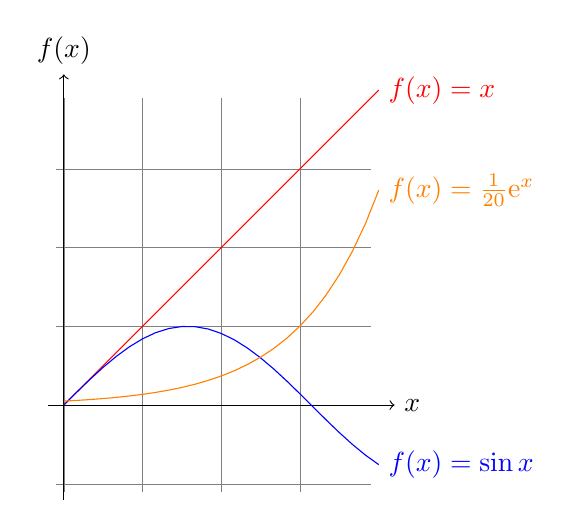
\begin{tikzpicture}[domain=0:4]
		  \draw[very thin,color=gray] (-0.1,-1.1) grid (3.9,3.9);
  		\draw[->] (-0.2,0) -- (4.2,0) node[right] {$x$};
		  \draw[->] (0,-1.2) -- (0,4.2) node[above] {$f(x)$};
		  \draw[color=red]    plot (\x,\x)             node[right] {$f(x) =x$};
  % \x r 表示弧度
		  \draw[color=blue]   plot (\x,{sin(\x r)})    node[right] {$f(x) = \sin x$};
		  \draw[color=orange] plot (\x,{0.05*exp(\x)}) node[right] {$f(x) = \frac{1}{20} \mathrm e^x$};
		\end{tikzpicture}
	%\end{center}
\end{minipage}



\begin{minipage}[htpb][80mm][t]{80mm}
	%\begin{center}
		\vspace*{60mm}
    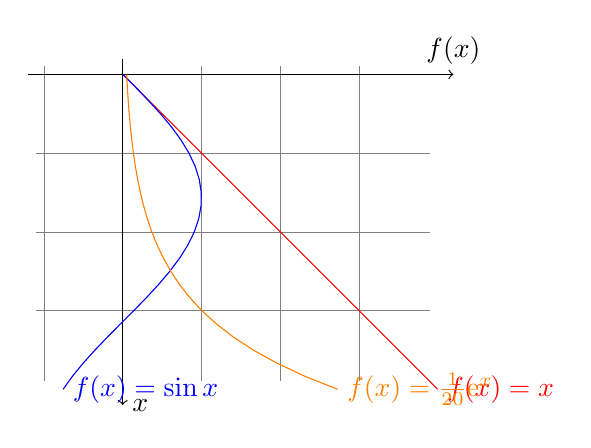
\begin{tikzpicture}[domain=0:4,scale=1,rotate=270]
		  \draw[very thin,color=gray] (-0.1,-1.1) grid (3.9,3.9);
  		\draw[->] (-0.2,0) -- (4.2,0) node[right] {$x$};
		  \draw[->] (0,-1.2) -- (0,4.2) node[above] {$f(x)$};
		  \draw[color=red]    plot (\x,\x)             node[right] {$f(x) =x$};
  % \x r 表示弧度
		  \draw[color=blue]   plot (\x,{sin(\x r)})    node[right] {$f(x) = \sin x$};
		  \draw[color=orange] plot (\x,{0.05*exp(\x)}) node[right] {$f(x) = \frac{1}{20} \mathrm e^x$};
		\end{tikzpicture}
	%\end{center}
\end{minipage}

% \chapter{公式測試}

\vskip 20 mm
\begin{minipage}[htpb]{80mm}
		\vspace*{45mm}
	%\begin{center}
			{\normalsize With normalsize 10 pt in class (truely 9.13\,pt in real dimen):
				\[ \sampleEq \]\par}

			{\Large With Large 14 pt in class (truely 12.782\,pt in real dimen):
				\[ \sampleEq \]\par}

			{\footnotesize With footnotesize 8 pt in class (truely 7.304\,pt in real dimen):
				\[ \sampleEq \]\par}
	%\end{center}
\end{minipage}

\clearpage
\begin{minipage}[htpb]{120mm}
		\vspace*{10mm}
	%\begin{center}
			{\normalsize 
				\[ \sampleEq \]\par}

			{\Large 
				\[ \sampleEq \]\par}

			{\footnotesize
				\[ \sampleEq \]\par}
	%\end{center}
\end{minipage}